% p10-06 例 2：等边 △ABC 内一点 P，PA=3, PB=4, PC=5；旋转 △APB 绕 B 顺时针 60° → △CP'B
% BC^2 = 25 + 12√3 → BC ≈ √45.78 ≈ 6.77
% 取 BC ≈ 6.77，建坐标 B(0,0), C(6.77, 0), A=(3.39, 5.87)
% P 满足 PB=4, PC=5, PA=3：用三角法可解
% 计算：PB=4, PC=5, BC=6.77 → 在 △PBC 中 cos∠PBC = (16+45.8-25)/(2·4·6.77)= 36.8/54.16 = 0.679 → ∠PBC ≈ 47.27°
% P = 4(cos47.27°, sin47.27°) = (2.71, 2.94)；P→A 距离验证：A-P=(0.68,2.93), |·|=3.01 ✓
% 旋转 △APB 绕 B 顺时针 60° (A→C)：P→P' 满足 BP'=4, ∠PBP'=60°
% P 极角 47.27°，顺时针 60° → P' 极角 -12.73°；P'=4(cos(-12.73°), sin(-12.73°))=(3.90, -0.88)
\documentclass[tikz,border=4pt]{standalone}
\usepackage{ctex}
\usepackage{amsmath}
\usetikzlibrary{calc, arrows.meta}
\begin{document}
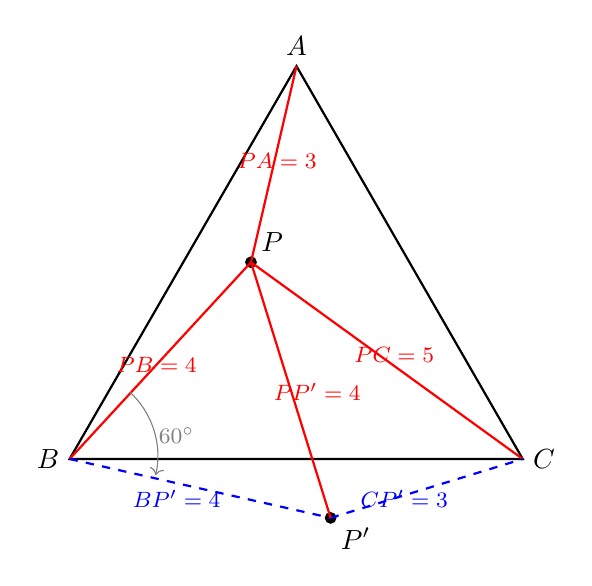
\begin{tikzpicture}[scale=0.85, thick]
  \coordinate (B) at (0,0);
  \coordinate (C) at (6.77, 0);
  \coordinate (A) at (3.39, 5.87);
  \coordinate (P) at (2.71, 2.94);
  \coordinate (Pp) at (3.90, -0.88);

  \draw (A)--(B)--(C)--cycle;
  \filldraw (P) circle (2pt) node[above right] {$P$};
  \filldraw (Pp) circle (2pt) node[below right] {$P'$};

  % PA, PB, PC
  \draw[red, thick] (P)--(A);
  \draw[red, thick] (P)--(B);
  \draw[red, thick] (P)--(C);

  % 旋转后 △BP'C（C 对应 A）
  \draw[blue, dashed, thick] (B)--(Pp);
  \draw[blue, dashed, thick] (Pp)--(C);
  % PP' = 4 (等边)
  \draw[red, thick] (P)--(Pp);

  \node[above] at (A) {$A$};
  \node[left]  at (B) {$B$};
  \node[right] at (C) {$C$};

  \node[font=\footnotesize, red] at (3.1, 4.45) {$PA=3$};
  \node[font=\footnotesize, red] at (1.3, 1.4) {$PB=4$};
  \node[font=\footnotesize, red] at (4.85, 1.55) {$PC=5$};
  \node[font=\footnotesize, blue] at (1.6, -0.6) {$BP'=4$};
  \node[font=\footnotesize, blue] at (5.0, -0.6) {$CP'=3$};
  \node[font=\footnotesize, red] at (3.7, 1.0) {$PP'=4$};

  % 旋转角 60°
  \draw[->, gray, thin] (0.9, 1.0) arc[start angle=47.27, end angle=-12.73, radius=1.3];
  \node[gray, font=\footnotesize] at (1.6, 0.35) {$60^\circ$};
\end{tikzpicture}
\end{document}
